\chapter{Introduction}
\lecture{1}{2 Sep. 13:20}{}
\section{Geometry}
\begin{itemize}
    \item linear
    \item To study geometry with linearity
    \item In a different dimension:
    \begin{itemize}
        \item In 2D: \textcolor{red}{\textbf{lines}}
        \item In 3D: \textcolor{red}{\textbf{planes}}
        \item In $n$D: \textcolor{red}{\textbf{hyperplanes}}

    \end{itemize}
\end{itemize}

\section{Abstract Algebra}

\begin{definition}[Linear Algebra]
    Here is the definition of Linear algebra.
    \begin{itemize}
        \item Algebra is the study of basic "mathematical structure." \\
        e.g. \textbf{Group}, \textbf{Ring}, \textbf{Field}, ...etc.
        \item Linear Algebra studies one of the structures called \textcolor{red}{\textbf{vector space}}.
    \end{itemize}
\end{definition}

\begin{note}
Followed by logical deduction from the basic definition, we can derive some theorems.
\end{note}

\section{Applied Science}
\begin{itemize}
    \item \textbf{Mathematic}: ODE, PDE.
    \item \textbf{Linear Programming}: developing during World War II
    \item \textbf{Imange Processing}, \textbf{Computer Vision}, \textbf{Computer Graphic}, etc.
\end{itemize}

\chapter{Matrices and Gaussian Elimination}
\section{Introduction}

The central problem of Linear Algebra is the solution of Linear Equations. The most important and simplest case is when the $\#$ of unknowns equals to the $\#$ of equations.

\begin{note}
There are two ways to solve linear equations:
\begin{itemize}
    \item The method of elimination \textbf{(Gaussian Elimination)}
    \item Determinants \textbf{(Crammer's Rule)}
\end{itemize}
\end{note}

\subsection{Four aspects to follow}
\begin{enumerate}[label=(\arabic*)]
    \item The geometry of linear equations.
    \begin{note}
        $n=2, n=3 \quad \rightarrow\quad$ higher dimensional space.
    \end{note}
    \item The interpretation of elimination is a factorization of the coefficient matrix.
    \begin{definition*}
        Some notation to define:
        \begin{definition}[Scalar, Matrix, Vector]
        \[
        Ax = b \qquad
        \begin{cases}
            \alpha, \beta, \gamma: &\text{scalar} \\
            A, B, C: &\text{matrix} \\
            a, b, c: &\text{vector}
        \end{cases}        
        \]
        \end{definition}
        \begin{definition}[Lower/Upper triangular matrix]
        \[
        A = LU \qquad
        \begin{cases}
            L: &\text{lower triangular matrix} \\
            U: &\text{upper triangular matrix}
        \end{cases}    
        \]
        \end{definition}
        \begin{definition}[Transpose/Inverse]
        \[
        A^T/A^{-1}: \qquad
        \begin{cases}
            A^T: &\text{Transpose of matrix A} \\
            A^{-1}: &\text{Inverse of matrix A}
        \end{cases}   
        \]
        \end{definition}
    \end{definition*}

    \newpage

    \item Irregular case and Singular case \textbf{(no unique solution)}:
    \begin{note}
        no solution or infinitely many solutions
    \end{note}
    \item \textbf{The $\#$ of operations to solve the system by elimination}
\end{enumerate}

\vspace{1em}

\section{Geometry of Linear Equation}

\begin{eg}
Consider the linear equation below:
    \[
    \begin{cases}
        2x-y&=1\\
        x+ y&=5
    \end{cases}
    \]
\end{eg}

\begin{itemize}
    \item \textbf{approach 1}: \textbf{row picture} $\rightarrow$ two lines in plane

    \begin{figure}[H]
        \centering
        \incfig[0.75\textwidth]{1.2.1}
        \caption{Row Picture}
        \label{fig:1.2.1}
    \end{figure}

    \item \textbf{approach 2}: \textbf{column picture}
    \begin{figure}[H]
        \centering
        \incfig[0.7\textwidth]{1.2.2}
        \caption{Column Picture}
        \label{fig:1.2.2}
    \end{figure}

    \begin{lemma}[Linear Combination]
    \[
    x
    \left(
    \begin{matrix}
    2 \\
    1
    \end{matrix}\right)
    +y
    \left(\begin{matrix}
    -1 \\
    1
    \end{matrix}\right)
    = 
    \left(\begin{matrix}
    1 \\
    5
    \end{matrix}\right)
    \]
    \end{lemma}

    \vspace{1.2em}
    
    To find the \textbf{Linear Combination} of  \(\left(
    \begin{matrix}
    2 \\
    1 
    \end{matrix}\right)\) and \(\left(
    \begin{matrix}
    -1 \\
    1 
    \end{matrix}\right)\) to reach \(\left(
    \begin{matrix}
    1 \\
    5 
    \end{matrix}\right)\)


\end{itemize}

\begin{note}
A vector is a $n\times1$ array with $n$ real numbers, $c_n$ is $$\left(\begin{matrix}
    c_1\\ \vdots \\ c_n
\end{matrix}\right)$$
But in the text, we use $$(c1, \cdots, c_n)$$ to represent.
\end{note}

\begin{definition*}
    Here are some operations on matrix:
    \begin{definition}
        \[
        \alpha \left(
        \begin{matrix}
            c_1\\ \vdots \\ c_n
        \end{matrix}
        \right)_{n\times1} = 
        \left(
        \begin{matrix}
            \alpha \cdot c_1\\ \vdots \\ \alpha \cdot c_n
        \end{matrix}
        \right)_{n\times1}, \qquad \alpha \in \mathbb{R}
        \]
    \end{definition}
    \begin{definition}
        \[
        \left(
        \begin{matrix}
            c_1\\ \vdots \\ c_n
        \end{matrix}
        \right) + 
        \left(
        \begin{matrix}
            d_1\\ \vdots \\ d_n
        \end{matrix}
        \right)
        = 
        \left(
        \begin{matrix}
            c_1+d_1\\ \vdots \\ c_n + d_n
        \end{matrix}
        \right)_{n\times1}
        \]
    \end{definition}
    \begin{definition}
        \[
        y \in \mathbb{R}
        \]
        \vspace{1pt}
        \[
        y \in \mathbb{R}^2 \ \Longrightarrow  \ y = \left(\begin{matrix}
           y_1 \\
           y_2
        \end{matrix}
        \right)_{2\times1}  \quad y_1, y_2 \in \mathbb{R}
        \]
        \vspace{1pt}
        \[
        y \in \mathbb{R}^3 \ \Longrightarrow  \ y = \left(\begin{matrix}
           y_1 \\
           y_2 \\
           y_3
        \end{matrix}
        \right)_{3\times1}  \quad y_1, y_2, y_3 \in \mathbb{R}
        \]
    \end{definition}
\end{definition*}

\newpage

\begin{eg}
    Consider the linear equation below:
    \[
    \begin{cases}
        2u +v +w&=5\\
        4u-6v &=-2 \\
        -2u + 7u + 2w &= 9
    \end{cases}
    \]
\end{eg}

\begin{itemize}
    \item Row picture

\begin{center}    
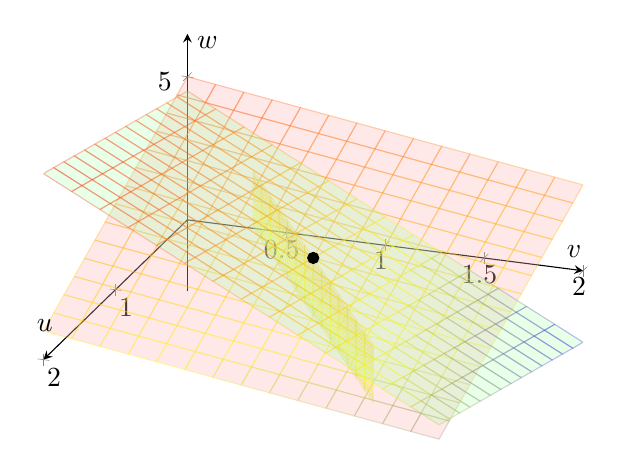
\begin{tikzpicture}
  \begin{axis}[
    axis lines=center,
    xlabel={$u$}, ylabel={$v$}, zlabel={$w$},
    view={110}{30},
    grid=major,
    samples=15,
    domain=0:2,        % 縮小範圍
    y domain=0:2,
  ]
    % 第一個平面: 2u + v + w = 5 → w = 5 - 2u - v
    \addplot3[surf, opacity=0.3, fill=red!30, shader=flat, draw=none] {5 - 2*x - y};

    % 第二個平面: 4u - 6v = -2 → v = (2 + 4u)/6
    \addplot3[surf, opacity=0.3, fill=Goldenrod!30, shader=flat, draw=none] 
      ({x}, {(2+4*x)/6}, {y});

    % 第三個平面: -2u + 7v + 2w = 9 → w = (9+2u-7v)/2
    \addplot3[surf, opacity=0.3, fill=green!30, shader=flat, draw=none] 
      ({x}, {y}, {(9+2*x-7*y)/2});

    % 解點 (交點)
    \addplot3[mark=*] coordinates {(1,1,2)};
  \end{axis}
\end{tikzpicture}
\end{center}
    \[
    (u, v, w) = (1, 1, 2)
    \]
    \begin{lemma}
        in $n$-dimension, a line require $(n-1)$ equation.
    \end{lemma}

    \begin{exercise}
        How to extend into $n$-dimensions?
    \end{exercise}
    \begin{answer}
    Consider the following steps:
        \begin{itemize}
            \item Each equation represents a plane or hyperplane.
            \item The first equation produces a $(n-1)$-dimension plane in $\mathbb{R}^n$
            \item The second equation produces another $(n-1)$-dimension plane in $\mathbb{R}^n$
            \item Their intersection in smaller set of $(n-2)$-dimension
            \item $(n-3) \rightarrow (n-4) \rightarrow \cdots\cdots \rightarrow 3 \rightarrow 2 \rightarrow 1 \rightarrow \text{point}$
        \end{itemize}

        Then we can find the final intersection.
    \end{answer}

    \item Column picture
    \[
    u \left(\begin{matrix}
        2 \\ 4 \\ -2
    \end{matrix}\right) + 
    v \left(\begin{matrix}
        1 \\ -6 \\ 7
    \end{matrix}\right) + 
    w \left(\begin{matrix}
        1 \\ 0 \\ 2
    \end{matrix}\right) = 
    \left(\begin{matrix}
        5 \\ -2 \\ 9
    \end{matrix}\right) \qquad \Longleftarrow \qquad
    \begin{cases}
        2u +v +w&=5\\
        4u-6v &=-2 \\
        -2u + 7u + 2w &= 9
    \end{cases}
    \]
    RHS is a linear combination of 3 column vectors.

    \begin{theorem}
    Solution to a linear equation:
    \[
    (\underset{\text{row pic.}}{\textbf{intersection of to points}}) \ = \ (\underset{\text{column pic.}}{\textbf{coefficient of linear combination}})
    \]
    \end{theorem}
\end{itemize}

\newpage

\subsection{Singular Case}

\begin{enumerate}[label=(\arabic*)]
    \item Row Picture: In 3D case, they didn't intersect at a point.
    \begin{itemize}
        \item \textbf{Case 1}: two parallel
        \[
        \begin{cases}
        2u +v +w&=5\\
        4u+2v+2w &=9 \\
        \end{cases}
        \]
        
        \item \textbf{Case 2}: three plane perpendicular ($\perp$)
        \[
        \begin{cases}
        u +v +w&=2 \ \cdots\ (1)\\
        2u+3w &=5 \ \cdots\ (2)\\
        3u+v+4w &= 6\ \cdots\ (3)\\
        \end{cases}
        \]
        \[
        \text{RHS} \Rightarrow (1)+(2)=(3)\quad ;\quad
        \text{LHS} \Rightarrow (1)+(2)\neq(3)
        \]
        
        \item \textbf{Case 2}: three plane have a whole line in common.
        \[
        \begin{cases}
        u +v +w&=2 \ \cdots\ (1)\\
        2u+3w &=5 \ \cdots\ (2)\\
        3u+v+4w &= 7\ \cdots\ (3)\\
        \end{cases}
        \]
        \[
        \text{RHS} \Rightarrow (1)+(2)=(3)\quad ;\quad
        \text{LHS} \Rightarrow (1)+(2)=(3)
        \]
        \item \textbf{Case 4}: three parallel
    \end{itemize}

    \item Column Picture:
    \[
    u\left(\begin{matrix}
    1 \\2 \\3
    \end{matrix}\right) + 
    v\left(\begin{matrix}
    1 \\0 \\1
    \end{matrix}\right) +
    w\left(\begin{matrix}
    1 \\3 \\4
    \end{matrix}\right) = 
    b
    \]

    In the case above, three vectors are linear combination to each other, i.e. three vectors share the same plane.
    
    \begin{lemma}[Singular case]
        If the three vectors are linear combination to each other (three vector share a common plane), it must be \textbf{singular case}.
        \begin{itemize}
            \item If \( b=
            \left(
            \begin{matrix}
                2 \\5 \\7
            \end{matrix}\right)
            \), which is on the plane \(\Rightarrow\) too many solution to produce $b$.
            \item If \( b=
            \left(
            \begin{matrix}
                2 \\5 \\6
            \end{matrix}\right)
            \), which is not on the plane \(\Rightarrow\) no solution.
        \end{itemize}
    \end{lemma}
\end{enumerate}

\newpage
\subsection{Fundamental Linear Algebra Theorem (Geometry form)}

\begin{theorem}[Fundamental LA Theorem]
Consider a linear system
\[
A x = b, \quad A \in \mathbb{R}^{m \times n}, \; x \in \mathbb{R}^n, \; b \in \mathbb{R}^m.
\]
If the $n$ hyperplanes have no only one intersection or infinitely many points, then the $n$ columns lie in the same plane. (consistency of \emph{row picture} and \emph{column picture})

\begin{notation} Logic notation:
    \begin{itemize}
        \item If ..., then : \(\implies\)
        \item If and only if : \(\iff\)
    \end{itemize}
\end{notation}
\end{theorem}